\documentclass{article}
\usepackage{graphicx}
\usepackage[svgnames,table]{xcolor}
\usepackage{booktabs}

\setlength\parindent{0pt}

\begin{document}
From the given data, the value of $\mathbf{\lambda}$ turns out to $\mathbf{0.70}$
\bigskip

And the table which compares observed relative
frequencies.

\rowcolors{2}{White}{LightBlue!30}
\medskip
\begin{tabular}{*3c}\toprule
	\textbf{Count of deaths} & \textbf{Fitted Poisson PMFs} & \textbf{Observed relative frequencies}\\
	\midrule
	0 & 139.043885 & 144 \\
	1 & 97.330720 & 91 \\
	2 & 34.065752 & 32 \\
	3 & 7.948675 & 11 \\
	4 & 1.391018 & 2 \\
	\bottomrule
\end{tabular}
\bigskip

And the plot:
\vspace{-9pt}

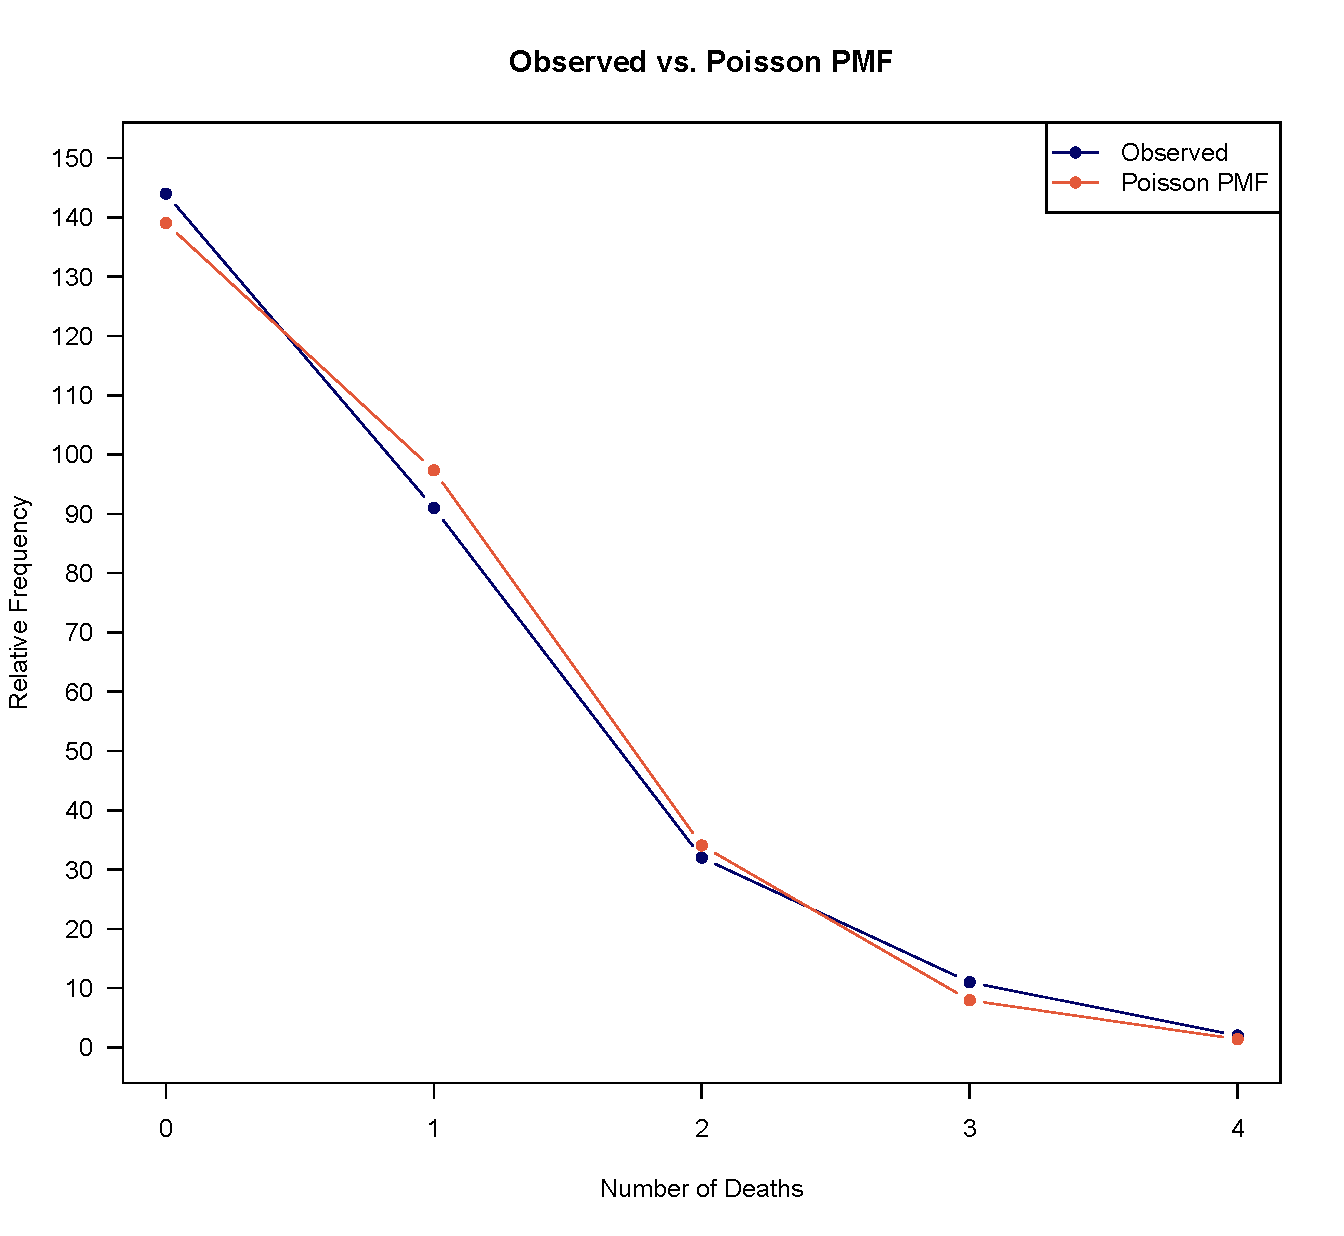
\includegraphics[width=12cm]{Q2-plot.pdf}

\end{document}
